% !TEX root = ../waves.tex
We recall here one the most important aspect of the previous chapter. We defined
trigonometric polynomials as arbitrary linear combinations of elementary waves with the
same period, explicitly
\begin{equation}
  P(t)=\frac{a_0}{2}+\sum_{n=1}^N[a_n\cw(t;n\omega)+b_n\sw(t;n\omega)]=
  \sum_{n=-N}^{N}c_n\ew(t;n\omega)\,.
\end{equation}
Then, we demonstrated that the coefficients defining $P$ are unique, and given by
\begin{align}
  a_n&=\frac{2}{\tau}\braket{P,\cw(n\omega)}
  =\frac{2}{\tau}\int_0^{\tau}\diff t\,P(t)\cos(2\pi n\omega t)\,,
  \label{eq:series-an-intro}\\
  b_n&=\frac{2}{\tau}\braket{P,\sw(n\omega)}
  =\frac{2}{\tau}\int_0^{\tau}\diff t\,P(t)\sin(2\pi n\omega t)\,,
  \label{eq:series-bn-intro}\\
  c_n&=\frac{1}{\tau}\braket{P,\ew(n\omega)}
  =\frac{1}{\tau}\int_0^{\tau}\diff t\,P(t)\,e^{-2\pi i n\omega t}\,,
  \label{eq:series-cn-intro}
\end{align}
where $\tau=\frac{1}{\omega}$. Those relationships were derived in the proofs
of~\cref{thm:trigp-unicity,corr:trigp-unicity-cplx}. Additionally, in~\cref{chap:wave-eq},
specifically~\cref{sec:toward-fourier}, we conjectured that solutions of the wave equation
can be written as an infinite sum of sine waves, and computed explicitly the coefficients
of this sum in the case of the plucked string, using~\cref{eq:wave-eq} which is very
similar to the expressions above.

In summary, what we found studying the wave equation suggests that some functions can be
approximated arbitrarily well by trigonometric polynomials. This expansion can be
conjectured by generalising the integrals above, replacing $P$ by an arbitrary function
$f$. If one defines $a_n$, $b_n$, and $c_n$ in that way, is the equation below correct?
\begin{equation}
  f(t)=\frac{a_0}{2}+\sumnp{n}[a_n\cw(t;n\omega)+b_n\sw(t;n\omega)]=
  \sumz{n}c_n\ew(t;n\omega)
\end{equation}
Answering accurately this question will be the main topic of this chapter.
%%%%%%%%%%%%%%%%%%%%%%%%%%%%%%%%%%%%%%%%%%%%%%%%%%%%%%%%%%%%%%%%%%%%%%%%%%%%%%%%%%%%%%%%%%
\section{Piecewise smooth functions}
As discussed in the next sections, the convergence of the Fourier expansion is a
non-trivial question, and it is sensitive on the regularity of the expanded function. In
this section we define a class of functions to study this question, which is general
enough to include most applications relevant to mathematical physics. Piecewise smooth
functions are essentially continuous and differentiable functions, except perhaps at a
finite number of points, with finite limits around discontinuities. We start by defining
this specific type of discontinuity.
\begin{definition}
  Let $f$ be a complex function of a single real variable. We consider a point $t_0\in\mathbb{R}$,
  and assume $f$, and let assume $f$ is defined in a neighbourhood of some point
  $t_0\in\mathbb{R}$. If $f(t)$ admits a finite limit for $t\to t_0$ with $t<t_0$, we call
  it the \emph{left limit} of $f(t)$ at $t_0$, noted $f(t_0^-)$. Similarly, if $f(t)$
  admits a finite limit for $t\to t_0$ with $t>t_0$, we call it the \emph{right limit} of
  $f(t)$ at $t_0$, noted $f(t_0^+)$. In general $f(t_0^-)$ and $f(t_0^+)$ are called
  \emph{one-sided} limits of $f$ at $t_0$.
\end{definition}
\begin{definition}
  Let $f$ be a complex function of a single real variable, which admits a left and right limits at
  a given point $t_0$. If $f(t_0^-)\neq f(t_0^+)$, then $t_0$ is called a \emph{jump
  discontinuity} of $f$, and the difference $f(t_0^+)-f(t_0^-)$ is called the
  \emph{height} of the jump discontinuity.
\end{definition}
\begin{example}
  The square wave function $\sq$ defined in~\cref{eq:wave-square} has jump discontinuities
  of height $2$ at all points $t$ such that $t=\frac{n}{2}$ where $n\in\mathbb{Z}$.
\end{example}
We now define \emph{piecewise continuous functions}, which are continuous functions,
perhaps at the exception to a finite number of jump discontinuities.
\begin{definition}
  \label{def:pw-cont}
  Let $f$ be a complex function of a single real variable defined on a compact interval $[a,b]$.
  $f$ is said to be \emph{piecewise continuous} is said to be on $[a,b]$ if there exists a
  finite set of points of $t_0=a<t_1<\dots<t_{N-1}<t_N=b$ in $(a,b)$ satisfying all the
  following conditions:
  \begin{itemize}
    \item[(PC1)] for all integers $n$ with $0\leq n< N$, $f$ is continuous on
      $(t_n,t_{n+1})$;
    \item[(PC2)] for all integers $n$ with $0< n< N$, $t_n$ is a jump discontinuity of
      $f$;
    \item[(PC3)] $f$ admits finite right and left limits in $a$ and $b$, respectively;
  \end{itemize}
  In particular, any continuous function on $[a,b]$ is piecewise continuous.
\end{definition}
\emph{Piecewise smooth} functions are then naturally defined by additionally requiring the
derivative to be piecewise continuous.
\begin{definition}
  \label{def:pw-smooth}
  Let $f$ be a complex function of a single real variable defined on a compact interval $[a,b]$.
  $f$ is said to be \emph{piecewise smooth} on $[a,b]$ if it is piecewise continuous and
  admits a derivative which is piecewise continuous.
\end{definition}
\begin{example}
  The square wave function $\sq$ is piecewise smooth.
\end{example}
\begin{example}
  The following function
  \begin{equation}
    f(t)=
    \begin{cases}
      \sqrt{t} & \text{if}~t\geq 0\\
      0 & \text{else}
    \end{cases}\,,
  \end{equation}
  is continuous, but it is not piecewise smooth. Indeed, its derivative for $t\neq 0$ is
  given by
  \begin{equation}
    f'(t)=
    \begin{cases}
      \frac{1}{2\sqrt{t}} & \text{if}~t>0\\
      0 & \text{if}~t<0
    \end{cases}\,.
  \end{equation}
  $f'(t)$ has a discontinuity at $0$ which is not a jump discontinuity since the right
  limit at this point diverges.
\end{example}
\begin{example}
  \label{ex:sininv}
  The function $f$ defined by $f(t)=\sin(\frac{1}{t})$ (represented in~\cref{ex:sininv})
  is continuously differentiable and bounded on $(0,1)$, however it does not admit a right
  limit at $t=0$, and therefore is not continuous on $[0,1]$.
\end{example}
\begin{example}
  The function $f$ defined by $f(t)=|t|$ is piecewise smooth on $[-1,1]$. Indeed, it is
  clearly continuous on $[-1,1]$, and its derivative for $t\neq 0$ is given by the
  \emph{sign function}
  \begin{equation}
    f'(t)=\sign(t)=\frac{t}{|t|}=
    \begin{cases}
      -1&~\mathrm{if}~t<0\\
      1&~\mathrm{if}~t>0
    \end{cases}\,.
  \end{equation}
  This function is continuous on $[-1,0)$ and $(0,1]$, and has a jump discontinuity of
  height $2$ at $t=0$ with the left and right limits
  \begin{equation}
    f'(0^-)=-1\qquad\text{and}\qquad f'(0^+)=1\,.
  \end{equation}
\end{example}
We now give a definition over the whole real line in the case of periodic functions.
\begin{definition}
  We say that a $\tau$-periodic function is piecewise continuous if it is piecewise
  continuous on a period, \eg it is piecewise continuous on $[0,\tau]$. Similarly, a
  $\tau$-periodic function is said to be piecewise continuous if it is piecewise smooth on
  a period.
\end{definition}
A first important property of piecewise smooth functions is their boundedness and
integrability.
\begin{proposition}
  A piecewise smooth function $f$ on $[a,b]$ is bounded on $[a,b]$, and has a bounded
  derivative $f'$. In particular, both $f$ and $f'$ are integrable on $[a,b]$.
\end{proposition}
\begin{proof}
  We reuse here the notations of~\cref{def:pw-cont}. For all $n$ with $0\leq n< N$, $f$ is
  continuous on $(t_n,t_{n+1})$ according to condition (PC1). Using conditions (PC2) and
  (PC3), $f$ admits right and left limits in $t_n$ and $t_{n+1}$, respectively. This
  implies $f$ admits a continuous extension on the compact interval $[t_n,t_{n+1}]$, and
  therefore is bounded on $[t_n,t_{n+1}]$. The same arguments can be applied to the
  derivative $f'$.
\end{proof}
\begin{figure}[t]
  \centering
  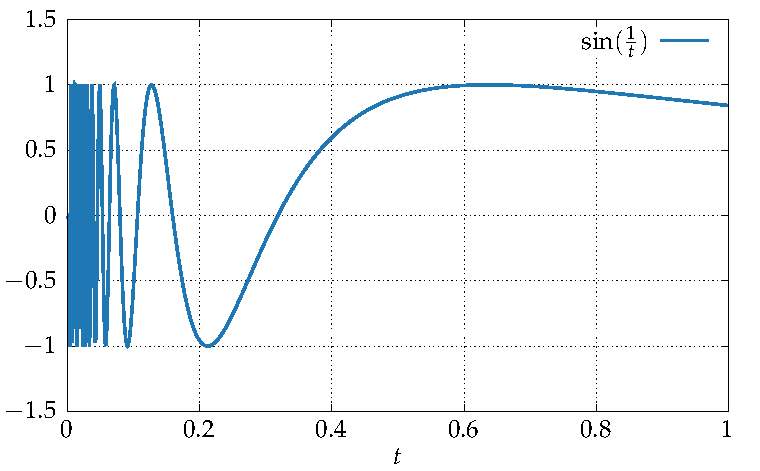
\includegraphics{gp_sininv.pdf}
  \caption{Curve of the function $f(t)=\sin(\frac{1}{t})$ from~\cref{ex:sininv}.}
  \label{fig:sininv}
\end{figure}
Finally, we show that the one-sided limits of the derivative of piecewise smooth functions
can be calculated with the usual limits:
\begin{proposition}
  \label{prop:oneside-der}
  Let $f$ be a piecewise smooth function on $[a,b]$, and let $t_0\in(a,b)$. The one-sided
  limits of $f'$ are given by the following limits
  \begin{equation}
    f'(t_0^-)=\lim_{\substack{h\to0\\h>0}}\frac{f(t_0^-)-f(t_0-h)}{h}
    \qquad\text{and}\qquad
    f'(t_0^+)=\lim_{\substack{h\to0\\h>0}}\frac{f(t_0+h)-f(t_0^+)}{h}
  \end{equation}
\end{proposition}
\begin{proof}
  Let $h>0$ small enough such that $t_0-h\in(a,b)$, and such that $f$ is continuously
  differentiable on $(t_0-h,t_0)$. Additionally, using condition (PC3)
  of~\cref{def:pw-cont}, $f$ restricted to $(t_0-h,t_0)$ can be extended to a continuous
  function on $[t_0-h,t_0]$ which take the value $f(t_0^-)$ in $t_0$. According to the
  mean value theorem, there exists $c_h$ in $(t_0-h,t_0)$ such that
  \begin{equation}
    f'(c_h)=\frac{f(t_0^-)-f(t_0-h)}{h}\,.
  \end{equation}
  Since $t_0-h<c_h<t_0$, then clearly $c_h\to t_0$ for $h\to 0$ with $h>0$, therefore
  \begin{equation}
    \lim_{\substack{h\to0\\h>0}}f'(c_h)=f'(t_0^-)
    =\lim_{\substack{h\to0\\h>0}}\frac{f(t_0^-)-f(t_0-h)}{h}\,.
  \end{equation}
  This proves the proposition for the left limit of $f'$. The right limit can be
  identically proven by considering the mean value theorem on a small interval
  $[t_0,t_0+h]$.
\end{proof}

%%%%%%%%%%%%%%%%%%%%%%%%%%%%%%%%%%%%%%%%%%%%%%%%%%%%%%%%%%%%%%%%%%%%%%%%%%%%%%%%%%%%%%%%%%
\section{Partial Fourier sums}
In this section, we formalise the generalisation of the
coefficients~\cref{eq:series-an-intro,eq:series-bn-intro,eq:series-cn-intro} mentioned in
the introduction to this section, as well as the associated trigonometric polynomials.
%.........................................................................................
\subsection{Fourier coefficients}
\begin{definition}
  \label{def:fourier-coef}
  Let $f$ be a piecewise smooth $\tau$-periodic function. We call \emph{cosine},
  \emph{sine}, and \emph{complex Fourier coefficients} the sequences
  \begin{align}
    a_n(f)&=\frac{2}{\tau}\braket{f,\cw(n\omega)}
    =\frac{2}{\tau}\int_0^{\tau}\diff t\,f(t)\cos(2\pi n\omega t)\,,\\
    b_n(f)&=\frac{2}{\tau}\braket{f,\sw(n\omega)}
    =\frac{2}{\tau}\int_0^{\tau}\diff t\,f(t)\sin(2\pi n\omega t)\,,\\
    c_n(f)&=\frac{1}{\tau}\braket{f,\ew(n\omega)}
    =\frac{1}{\tau}\int_0^{\tau}\diff t\,f(t)\,e^{-2\pi i n\omega t}\,,
  \end{align}
  respectively, where $n\in\mathbb{Z}$ and $\omega=\frac{1}{\tau}$.
\end{definition}
\begin{definition}
  \label{def:fourier-partial}
  Let $f$ be a piecewise smooth $\tau$-periodic function. For any integer $N\geq 0$, we
  call \emph{partial Fourier sum} of degree $N$ the trigonometric polynomial defined by
  \begin{equation}
    s_N(f)=\frac{a_0(f)}{2}+\sum_{n=1}^N[a_n(f)\cw(n\omega)+b_n(f)\sw(n\omega)]=
    \sum_{n=-N}^{N}c_n(f)\ew(n\omega)\,,
  \end{equation}
  where $\omega=\frac{1}{\tau}$.
\end{definition}
Since we aim at studying the convergence of Fourier sums for $N\to+\infty$, an important
question is the asymptotic behaviour of Fourier coefficients for $n\to+\infty$, discussed
in the next section.
%.........................................................................................
\subsection{Riemann-Lebesgue lemma}
For a fairly general class of functions, it can be shown that these coefficients converge
to $0$ for $n\to+\infty$. This is a crucial result in Fourier analysis generally called
the~\emph{Riemann-Lebesgue lemma}, and a necessary condition for the convergence of
Fourier series. We prove this result below for piecewise continuous functions on compact
intervals.
\begin{theorem}[Riemann-Lebesgue lemma]
  \label{thm:rl}
  Let $f$ be a piecewise continuous function on a compact interval $[a,b]$. We have the
  following limit
  \begin{equation}
    \lim_{k\to+\infty}\int_a^b\diff t\, f(t)\sin(kt)=0
  \end{equation}
\end{theorem}
\begin{proof}
  The proof of this theorem is rather abstract and technical, but it is based on a fairly
  intuitive idea. A first observation one can make is that the Riemann-Lebesgue lemma is
  easily demonstrated for constant functions. Indeed, for any constant $A\in\mathbb{R}$
  \begin{equation}
    \int_a^b\diff t\,A\sin(kt)=\frac{A}{k}\,[\cos(ka)-\cos(kb)]\,.
    \label{eq:rl-const}
  \end{equation}
  Then $|\cos(ka)-\cos(kb)|<2$ for all $k\in\mathbb{R}$, so the integral above clearly
  converges to $0$ for $k\to+\infty$. In the general case where $f$ is piecewise
  continuous, $f$ is an assembly of bounded continuous functions. Such functions can be
  approximated arbitrarily well by piecewise constant functions, similarly to what is done
  when approximating an integral with rectangles. With such a construction, the simple
  example above with constant functions is then all that is needed to prove the theorem.
  Let us proceed with justifying this approach in details.

  Reusing the notation of~\cref{def:pw-cont}, we have
  \begin{equation}
    \int_a^b\diff t\, f(t)\sin(kt)
    =\sum_{n=0}^{N}\int_{t_n}^{t_{n+1}}\diff t\, f(t)\sin(kt)\,.
    \label{eq:pw-int}
  \end{equation}
  The function $f$ is piecewise continuous, so according to condition (PC1)
  of~\cref{def:pw-cont}, for a given integer $n$ such that $0\leq n<N$, $f$ is continuous
  on $(t_n,t_{n+1})$. Additionally, conditions (PC2) and (PC3) imply that $f$ admits
  finite right and left limits in $t_n$ and $t_{n+1}$, respectively. Therefore, the
  restriction of $f$ to $(t_n,t_{n+1})$ can be extended to a continuous function on the
  compact interval $[t_n,t_{n+1}]$. Now, continuous functions on compact intervals are
  uniformly continuous, \ie for all $\epsilon>0$, there exists $\delta>0$ such that for
  all pairs $x,y$ in $[t_n,t_{n+1}]$, $|x-y|<\delta$ implies that $|f(x)-f(y)|<\epsilon$.
  Let us subdivide the interval $[t_n,t_{n+1}]$ into $M$ points
  $r_0=t_n<r_1<\dots<r_{M-1}<r_M=t_{n+1}$ such that for all $m$ with $0\leq m<M$,
  $|r_{n+1}-r_n|<\eta$. We then define the piecewise constant function $g$ equal to the
  constant $f(r_m)$ on $[r_m,r_{m+1})$, and $g(r_N)=f(r_{N-1})$. For a given point
  $t\in(t_n,t_{n+1})$, there exists $m$ such that $t\in[r_m,r_{m+1})$, and therefore
  \begin{equation}
    |f(t)-g(t)|=|f(t)-f(r_m)|<\epsilon\,,
  \end{equation}
  since by construction $|t-r_m|<\delta$. We can now write
  \begin{equation}
    \int_{t_n}^{t_{n+1}}\diff t\, f(t)\sin(kt)
    =\int_{t_n}^{t_{n+1}}\diff t\, [f(t)-g(t)]\sin(kt)
    +\int_{t_n}^{t_{n+1}}\diff t\,g(t)\sin(kt)\,.
  \end{equation}
  The integral of $g$ above can be dealt with easily, as anticipated in the introduction
  of the proof, explicitly
  \begin{equation}
    \int_{t_n}^{t_{n+1}}\diff t\,g(t)\sin(kt)
    =\frac{1}{k}\sum_{m=0}^{M-1}f(r_m)[\cos(kr_m)-\cos(kr_{m+1})]\,,
  \end{equation}
  so
  \begin{equation}
    \lim_{k\to0}\,\int_{t_n}^{t_{n+1}}\diff t\,g(t)\sin(kt)=0\,.
    \label{eq:rl-intg}
  \end{equation}
  Now, using the triangle inequality,
  \begin{equation}
    \left|\int_{t_n}^{t_{n+1}}\diff t\, [f(t)-g(t)]\sin(kt)\right|<
    \int_{t_n}^{t_{n+1}}\diff t\, |f(t)-g(t)|<(t_{n+1}-t_n)\epsilon\,.
  \end{equation}
  Since $\epsilon$ can be chosen arbitrarily small, the inequality above implies that
  \begin{equation}
    \lim_{k\to0}\,\int_{t_n}^{t_{n+1}}\diff t\, [f(t)-g(t)]\sin(kt)=0\,.
    \label{eq:rl-intfmg}
  \end{equation}
  Combining~\cref{eq:rl-intg,eq:rl-intfmg}, we just proved that every term in the sum
  in~\cref{eq:pw-int} converges to $0$ for $k\to+\infty$, which demonstrates the theorem.
\end{proof}
\begin{figure}[t]
  \centering
  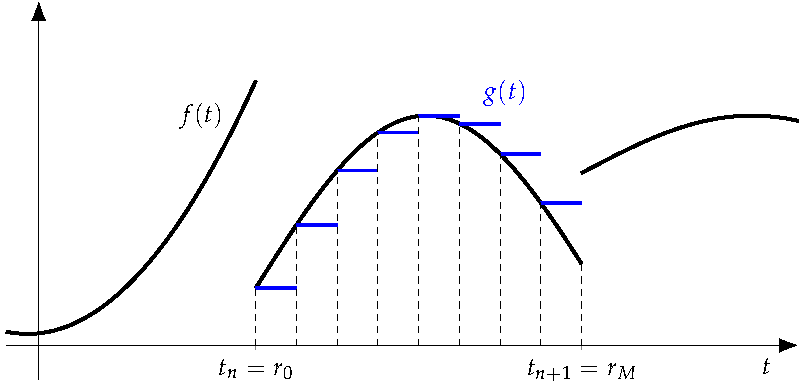
\includegraphics{tikz_rl.pdf}
  \caption{Illustration of the construction used in the proof of~\cref{thm:rl}
    (Riemann-Lebesgue lemma). The black curve represents an arbitrary piecewise continuous
    function, with visible jump discontinuities at $t_n$ and $t_{n+1}$. The blue lines
    represent a piecewise constant approximation $g$ of $f$ on the interval
  $[t_n,t_{n+1}]$, as defined in the proof of~\cref{thm:rl}}
  \label{fig:rl}
\end{figure}
\begin{corollary}
  Let $f$ be a function on $\mathbb{R}$ piecewise smooth on a compact interval $[a,b]$. We
  have the following limits
  \begin{align}
    \lim_{k\to+\infty}\int_a^b\diff t\, f(t)\cos(kt)&=0\,,\\
    \lim_{k\to+\infty}\int_a^b\diff t\, f(t)\,e^{ikt}=0
  \end{align}
\end{corollary}
\begin{proof}
  One can inspect the proof of~\cref{thm:rl} and notice that the only dependency on the
  $\sin(kt)$ weight in the integral comes from~\cref{eq:rl-const}. So it is sufficient to
  just repeat that step for the cosine function. We have
  \begin{equation}
    \int_a^b\diff t\, f(t)\cos(kt)=\frac{1}{k}[\sin(bk)-\sin(ak)]\,,
  \end{equation}
  and since $|\sin(bk)-\sin(ak)|<2$ for all $k\in\mathbb{R}$, the integral above vanishes
  for $k\to+\infty$. A similar argument can be made for the complex exponential, although
  one can also notice that it is now a trivial consequence the equality
  \begin{equation}
    \int_a^b\diff t\, f(t)\,e^{ikt}
    =\int_a^b\diff t\, f(t)\cos(kt)+i\int_a^b\diff t\, f(t)\sin(kt)\,.
  \end{equation}
\end{proof}
\begin{corollary}
  Let $f$ be a piecewise smooth $\tau$-periodic function. All the Fourier coefficients of
  $f$ converge to $0$, explicitly
  \begin{equation}
    \lim_{n\to+\infty}a_n(f)=\lim_{n\to+\infty}b_n(f)=\lim_{n\to+\infty}c_n(f)=0\,.
  \end{equation}
\end{corollary}
\begin{proof}
  This is a trivial consequence of the Riemann-Lebesgue lemma applied
  to~\cref{def:fourier-coef}.
\end{proof}
%.........................................................................................
\subsection{Dirichlet kernel}
In this section, we discuss a special function called the \emph{Dirichlet kernel}. This
function allows to write the partial Fourier sums as an integral (and as we will see in
later chapters, a convolution product), which is often used in combination with the
Riemann-Lebesgue lemma to demonstrate theorems on the convergence of Fourier series.
\begin{definition}
  We call~\emph{Dirichlet kernel} of degree $N$ the trigonometric polynomial defined by
  \begin{equation}
    D_N(x)=\sum_{n=-N}^{N}e^{inx}\,,\label{eq:dk-def}
  \end{equation}
  for any real number $x$. The Dirichlet kernel is by construction even and periodic with
  fundamental period $2\pi$.
\end{definition}
The Dirichlet kernel can in fact be expressed as a simple ratio of sine functions as
discussed in the result below.
\begin{proposition}
  \label{prop:dirichlet-id}
  For all $x\in\mathbb{R}$, and all $N\in\mathbb{N}$, we have
  \begin{equation}
    D_N(x)=1+2\sum_{n=1}^{N}\cos(nx)=\frac{\sin[(N+\frac{1}{2})x]}{\sin(\frac{x}{2})}\,.
    \label{eq:dk-sinratio}
  \end{equation}
\end{proposition}
\begin{proof}
  We start by defining the complex number $z$ by
  \begin{equation}
    z=\sum_{n=0}^Ne^{inx}\,.
  \end{equation}
  The Dirichlet kernel can then be written as follows:
  \begin{equation}
    D_N(x)=(z-1)^*+z=z^*+z-1=2\Re(z)-1=1+2\sum_{n=1}^{N}\cos(nx)\,,\label{eq:dk-z}
  \end{equation}
  which proves the first equality in~\cref{eq:dk-sinratio}. Since $e^{inx}=(e^{ix})^n$, we
  can simplify $z$ using a geometric sum:
  \begin{equation}
    z=\frac{e^{i(N+1)x}-1}{e^{ix}-1}\,.\label{eq:dk-geosum}
  \end{equation}
  We now have to compute the real part of $z$, let us start by rewriting the equation
  above to have a real denominator:
  \begin{equation}
    z=e^{-i\frac{x}{2}}\frac{e^{i(N+1)x}-1}{e^{i\frac{x}{2}}-e^{-i\frac{x}{2}}}
    =\frac{e^{i(N+\frac12)x}-e^{-i\frac{x}{2}}}{2i\sin(\frac{x}{2})}
    =-\frac{i}{2}\frac{e^{i(N+\frac12)x}-e^{-i\frac{x}{2}}}{\sin(\frac{x}{2})}\,,
  \end{equation}
  which has the real part
  \begin{equation}
    \Re(z)=\frac12\frac{\Im[e^{i(N+\frac12)x}]-\Im(e^{-i\frac{x}{2}})}{\sin(\frac{x}{2})}
    =\frac12\frac{\sin[(N+\frac{1}{2})x]}{\sin(\frac{x}{2})}+1\,.
  \end{equation}
  Substituting the last equation into~\cref{eq:dk-z} proves the proposition.
\end{proof}
\begin{proposition}
  \label{prop:dk-int}
  The Dirichlet kernel has the following integral on $[0,2\pi]$ for all $N\in\mathbb{N}$:
  \begin{equation}
    \int_0^{2\pi}\diff x\,D_N(x)=2\pi\,.
  \end{equation}
\end{proposition}
\begin{proof}
  Using~\cref{thm:orth-complex} with $m=0$ and $\tau=2\pi$, we obtain
  \begin{equation}
    \int_{0}^{2\pi}\diff x\,e^{inx}=2\pi\,\delta_{n0}\,,
  \end{equation}
  which substituted into~\cref{eq:dk-def} directly proves the proposition.
\end{proof}
We now formulate the main theorem on the integral representation of partial Fourier sums.
\begin{theorem}
  \label{thm:fourier-dk-rep}
  Let $f$ be a piecewise smooth $\tau$-periodic function. For all $N\in\mathbb{N}$, the
  partial Fourier sum of $f$ has the following integral representation:
  \begin{equation}
    s_N(f)(t)=\frac{1}{\tau}\int_0^{\tau}\diff u\,f(u)\,D_N[2\pi\omega(t-u)]\,.
  \end{equation}
\end{theorem}
\begin{proof}
  Using~\cref{def:fourier-coef,def:fourier-partial}, the partial Fourier sum $s_N(f)$ is
  given by
  \begin{equation}
    s_N(f)(t)=\frac{1}{\tau}\sum_{n=-N}^{N}e^{2\pi i n\omega t}
    \int_0^\tau\diff u\,f(u)e^{-2\pi i n\omega u}\,.
  \end{equation}
  Since the sum above is finite, we can exchange the sum and the integral to obtain
  \begin{equation}
    s_N(f)(t)=\frac{1}{\tau}\int_0^\tau\diff u\,f(u)\sum_{n=-N}^{N}e^{2\pi i n\omega (t-u)}\,.
  \end{equation}
  Finally, using the definition of the Dirichlet kernel~\cref{eq:dk-def} proves the
  theorem.
\end{proof}
%%%%%%%%%%%%%%%%%%%%%%%%%%%%%%%%%%%%%%%%%%%%%%%%%%%%%%%%%%%%%%%%%%%%%%%%%%%%%%%%%%%%%%%%%%
\section{Convergence of the Fourier expansion}
Using results from the previous section, we are now ready to discuss in details the
convergence of Fourier series. We start by discussing pointwise convergence, in a context
close to the original work of Peter Gustav Lejeune Dirichlet and Camille Jordan in the
second half of the 19\textsuperscript{th}, who brought stronger mathematical foundations
to the pioneering work of Fourier. We will then discuss the much stronger case of uniform
convergence, and conclude the section with the Gibbs phenomenon, which describes important
practical consequences of Fourier series which fail to converge uniformly.
%-----------------------------------------------------------------------------------------
\subsection{Pointwise convergence}
The theorem below can be considered as the main result of this chapter. It states that for
piecewise smooth periodic functions, the Fourier series converges at every point to the
average of the left and right limits. The essence of this theorem is that the Fourier
series does converge back to a given piecewise smooth periodic function, expect perhaps at
a finite number of points of jump discontinuity.
\begin{theorem}
  \label{thm:fourier-pt}
  Let $f$ be a $\tau$-periodic function which is piecewise smooth on $[0,\tau]$. For all
  $t\in\mathbb{R}$, the Fourier series for $f(t)$ converges with the following limit
  \begin{equation}
    \sumz{n}c_n(f)\,e^{2\pi i \omega nt}=\lim_{N\to+\infty}s_N(f)(t)
    =\frac{f(t^-)+f(t^+)}{2}\,.
  \end{equation}
  In particular, the Fourier series converges to $f(t)$ if $f$ is continuous in $t$.
\end{theorem}
\begin{proof}
  Let $t$ be a point in $[0,\tau]$. Using~\cref{thm:fourier-dk-rep}, we can write the
  partial Fourier sum $s_N(f)$ at the point $t$ as
  \begin{equation}
    s_N(f)(t)=\frac{1}{\tau}\int_{-\frac{\tau}{2}}^{\frac{\tau}{2}}\diff u\,
    f(u)\,D_N[2\pi\omega(t-u)]\,,
  \end{equation}
  where $\omega=\frac{1}{\tau}$, and the integration domain was shifted to
  $(-\frac{\tau}{2},\frac{\tau}{2})$, which is allowed by the $\tau$-periodicity of the
  integrand. We additionally perform the change of variable $u\mapsto t-u$ to obtain
  \begin{equation}
    s_N(f)(t)=\frac{1}{\tau}\int_{-\frac{\tau}{2}}^{\frac{\tau}{2}}\diff u\,
    f(t-u)\,D_N(2\pi\omega u)\,.
  \end{equation}
  Now, using~\cref{prop:dk-int}, we get
  \begin{equation}
    \int_{-\frac{\tau}{2}}^{\frac{\tau}{2}}\diff u\,D_N(2\pi\omega u)
    =\frac{\tau}{2\pi}\int_{-\pi}^{\pi}\diff x\,D_N(x)=
    \frac{\tau}{2\pi}\int_{0}^{2\pi}\diff x\,D_N(x)=\tau\,,
    \label{eq:fthm-partsum}
  \end{equation}
  where we used the change of variable $x=2\pi\omega u$, as well as the $2\pi$-periodicity
  of the Dirichlet kernel. Similarly, since $D_N(x)$ is even, we can write
  \begin{equation}
    \int_{0}^{\frac{\tau}{2}}\diff u\,D_N(2\pi\omega u)
    =\int_{-\frac{\tau}{2}}^{0}\diff u\,D_N(2\pi\omega u)=\frac{\tau}{2}\,.
  \end{equation}
  Since $f(t^-)$ and $f(t^+)$ are just constants, we can write
  \begin{align}
    \frac{f(t^-)}{2}&=\frac{1}{\tau}\int_{0}^{\frac{\tau}{2}}\diff u\,
    f(t^-)D_N(2\pi\omega u)\,,
    \label{eq:fthm-tmint}\\
    \frac{f(t^+)}{2}&=\frac{1}{\tau}\int_{-\frac{\tau}{2}}^{0}\diff u\,
    f(t^+)D_N(2\pi\omega u)\,.
    \label{eq:fthm-tpint}
  \end{align}
  We consider the two following integrals
  \begin{align}
    I^-_N&=\frac{1}{\tau}\int_{0}^{\frac{\tau}{2}}\diff u\,
    [f(t-u)-f(t^-)]D_N(2\pi\omega u)\,,\\
    I^+_N&=\frac{1}{\tau}\int_{-\frac{\tau}{2}}^{0}\diff u\,
    [f(t-u)-f(t^+)]D_N(2\pi\omega u)\,.
  \end{align}
  Using~\cref{eq:fthm-partsum,eq:fthm-tmint,eq:fthm-tpint}, we get
  \begin{equation}
    I^-_N+I^+_N=s_N(f)(t)-\frac{f(t^-)+f(t^+)}{2}\,.
    \label{eq:fourier-imip}
  \end{equation}
  Therefore, if we can show that $I^-_N$ and $I^+_N$ converge to $0$ for $N\to+\infty$,
  then the theorem is proven. Let us start by discussing $I^-_N$.
  Using~\cref{prop:dirichlet-id}, we can write
  \begin{equation}
    I^-_N=\frac{1}{\tau}\int_{0}^{\frac{\tau}{2}}\diff u\,
    \varphi^-(u)\sin\left[\left(N+\frac{1}{2}\right)2\pi\omega u\right]\,,
  \end{equation}
  where $\varphi^-$ is the function defined on all $u\in(0,\frac{\tau}{2})$ by
  \begin{equation}
    \varphi^-(u)=\frac{f(t-u)-f(t^-)}{\sin(\pi\omega u)}
    =\frac{f(t-u)-f(t^-)}{u}\frac{u}{\sin(\pi\omega u)}\,.
  \end{equation}
  If we can prove that $\varphi^-$ is piecewise continuous on
  $\smash{[0,\frac{\tau}{2}]}$, then $I^-_N$ converging to zero for $N\to+\infty$ is a
  direct consequence of the Riemann-Lebesgue lemma. Since $\sin(\pi\omega u)\neq 0$ for
  all $u\in\smash{(0,\frac{\tau}{2}]}$, and $f$ is piecewise smooth, the formula above
  clearly satisfies conditions (PC1) and (PC2) of~\cref{def:pw-cont}. However, it has an
  apparent singularity at $u=0$ that needs to be discussed for (PC3) to hold. For $u\to
  0$, $\sin(\pi\omega u)=\pi\omega u+\mathcal{O}(u^2)$ and therefore
  \begin{equation}
    \lim_{u\to 0}\,\frac{u}{\sin(\pi\omega u)}=\frac{1}{\pi\omega}\,.
  \end{equation}
  Then, using~\cref{prop:oneside-der}, we obtain
  \begin{equation}
    \lim_{\substack{u\to0\\u>0}}\varphi^-(u)=-\frac{f'(t^-)}{\pi\omega}\,,
  \end{equation}
  So $\varphi^-$ has a well-defined right limit for $u\to 0$, condition (PC3) is
  satisfied, $\varphi^-$ is piecewise continuous on $\smash{[0,\frac{\tau}{2}]}$,
  and~\cref{thm:rl} implies that
  \begin{equation}
    \lim_{N\to+\infty}I^-_N=0\,.
  \end{equation}
  We similarly write $I_N^+$ as
  \begin{equation}
    I^+_N=\frac{1}{\tau}\int_{-\frac{\tau}{2}}^{0}\diff u\,
    \varphi^+(u)\sin\left[\left(N+\frac{1}{2}\right)2\pi\omega u\right]\,,
  \end{equation}
  where
  \begin{equation}
    \varphi^+(u)=\frac{f(t-u)-f(t^+)}{\sin(\pi\omega u)}\,.
  \end{equation}
  As above, the limit
  \begin{equation}
    \lim_{\substack{u\to0\\u<0}}\varphi^+(u)=\frac{f'(t^+)}{\pi\omega}
  \end{equation}
  shows that $\varphi^+$ is piecewise continuous on $\smash{[-\frac{\tau}{2},0]}$, and
  therefore
  \begin{equation}
    \lim_{N\to+\infty}I^+_N=0\,.
  \end{equation}
  Coming back to~\cref{eq:fourier-imip}, the theorem is proven.
\end{proof}
\begin{example}
  The Fourier series of the square wave $\sq$ defined in~\cref{eq:wave-square} converges
  to the function
  \begin{equation}
    \sumz{n}c_n(\sq)\,e^{2\pi i \omega nt}=
    \begin{cases}
      1&\text{if}~0<t<\frac{1}{2}\\
      -1&\text{if}~\frac{1}{2}<t<-1\\
      \frac{1}{2}&\text{if}~t=0,\frac{1}{2},1
    \end{cases}\,,
  \end{equation}
  where it is understood that these values are repeated on every period. This limit is
  identical to the square wave except at the points of discontinuity where it takes the
  value $\frac{1}{2}$.
\end{example}
%-----------------------------------------------------------------------------------------
\subsection{Convergence in mean square and Parseval's theorem}
Another useful form of convergence for sequences of functions is the \emph{convergence in mean square}, also called \emph{$L^2$ convergence}, based on the functional norm introduced in~\cref{sec:ew-orth}. In all this section, we will work with square-integrable $\tau$-periodic functions. Such a function $f$ is defined by requiring that $|f|^2$ has a defined finite integral on $[0,\tau]$. This is the general class of functions for which the dot product is well-defined, which we will admit here. In particular, all piecewise smooth functions are square-integrable.
\begin{definition}
  Let $f$ be a $\tau$-periodic square-integrable function. A sequence of $\tau$-periodic square-integrable functions $f_n$ is said to converge to $f$ \emph{in mean} if
  \begin{equation}
    \lim_{n\to+\infty}\|f-f_n\|=0\,.
  \end{equation}
\end{definition}
This type of convergence is useful because the norm is related to the dot product of functions,
and as we saw in the previous chapter, the orthogonality of elementary waves. However, it is important to notice that this is a rather weak form of convergence, and without further assumptions it does not generally imply pointwise or uniform convergence.

We now generalise some results of~\cref{sec:ew-orth}, which we will then use to prove that Fourier series generally converge in mean square. Firstly, it is not too difficult to
show that the norm of a partial Fourier sum is always smaller than the norm of the associated function,
an important result known as \emph{Bessel's inequality}.
\begin{theorem}[Bessel's inequality]
  \label{thm:bessel}
  Let $f$ be a piecewise smooth $\tau$-periodic function. The series over $n\in\mathbb{Z}$
  with summand $|c_n(f)|^2$ converges, and one has the inequality
  \begin{equation}
    \tau\sumz{n}|c_n(f)|^2\leq\|f\|^2\,.
  \end{equation}
\end{theorem}
\begin{proof}
  We consider the norm of the difference between $f$ and its partial Fourier sum
  \begin{equation}
    \Delta_N=\|f-s_N(f)\|^2\,,
  \end{equation}
  where $N$ is some positive integer. By construction, $\Delta_N\geq 0$ for all $N>0$.
  Additionally, $\Delta_N$ can be expanded as
  \begin{align}
    \Delta_N&=\braket{f-s_N(f),f-s_N(f)}\\
    &=\|f\|^2+\|s_N(f)\|^2-2\Re[\braket{f,s_N(f)}]\,.\label{eq:bessel-l2err}
  \end{align}
  Furthermore,
  \begin{align}
    \braket{f,s_N(f)}&=\Braket{f,\sum_{n=-N}^{N}c_n(f)\ew(n\omega)}\\
    &=\sum_{n=-N}^{N}c_n(f)^*\braket{f,\ew(n\omega)}\\
    &=\tau\sum_{n=-N}^{N}|c_n(f)|^2\,.
  \end{align}
  Using Parseval's theorem for trigonometric polynomials (\cref{thm:trigp-parseval}), the result
  above implies that $\braket{f,s_N(f)}=\|s_N(f)\|^2$. Substituting this expression back into
  \cref{eq:bessel-l2err}, we get
  \begin{equation}
    \Delta_N=\|f\|^2-\|s_N(f)\|^2\,,
  \end{equation}
  and since $\Delta_N\geq 0$,
  \begin{equation}
    \forall N>0,\quad \|s_N(f)\|^2=\tau\sum_{n=-N}^{N}|c_n(f)|^2\leq \|f\|^2\,.
  \end{equation}
  $\|s_N(f)\|^2$ is a sum of positive numbers, and therefore a monotonous sequence in $N$. As per the inequality above, it is bounded by $\|f\|^2$ and therefore converges, which proves the theorem.
\end{proof}
In reality, this inequality is an equality, generalising~\cref{thm:trigp-parseval}. This is a much harder result to prove, and we will admit it here.
\begin{theorem}[Parseval]
  \label{thm:parseval}
  Let $f$ and $g$ be two square-integrable $\tau$-periodic functions. The following identities hold
  \begin{align}
    \braket{f,g}&=\tau\sumz{n}c_n(f)c_n(g)^*\,,
    \label{eq:fs-dot}\\
    \|f\|^2&=\tau\sumz{n}|c_n(f)|^2\,.
    \label{eq:fs-norm}
  \end{align}
\end{theorem}
For completeness, we provide below the Parseval theorem identities for the sine-cosine form
\begin{align}
  \braket{f,g}&=\tau\,\frac{a_0(f)a_0(g)^*}{4}
  +\frac{\tau}{2}\left\{\sumnp{n}[a_n(f)a_n(g)^*+b_n(f)b_n(g)^*]\right\}\,,\\
  \|f\|^2&=\tau\,\frac{|a_0(f)|^2}{4}+\frac{\tau}{2}\left\{\sumnp{n}[|a_n(f)|^2+|b_n(f)|^2]\right\}\,.
\end{align}
\begin{theorem}
  Let $f$ be a square-integrable $\tau$-periodic function. The Fourier series of $f$
  converges to $f$ in mean.
\end{theorem}
\begin{proof}
  We need to show that
  \begin{equation}
    \Delta_N =\|f-s_N(f)\|^2
  \end{equation}
  converges to $0$ for $N\to+\infty$. As already demonstrated in the proof of~\cref{thm:bessel},
  \begin{equation}
    \Delta_N =\|f\|^2-\tau\sum_{n=-N}^{N}|c_n(f)|^2\,.\label{eq:l2cvg-deltan}
  \end{equation}
  Using Parseval's theorem, we know that
  \begin{equation}
    \lim_{N\to+\infty}\tau\sum_{n=-N}^{N}|c_n(f)|^2=\|f\|^2\,,
  \end{equation}
  which applied to~\cref{eq:l2cvg-deltan} proves the theorem.
\end{proof}
The proof above is quite simple once one knows Parseval's theorem. In fact, Parseval's theorem
is truly the non-trivial property here, and it can be shown to be a necessary and sufficient condition
to the convergence in mean square. Proving Parseval's theorem it quite technical and out of the scope of this introductory course, however we will sketch the proof in the next section.
\subsection{Uniform convergence}
We start by reminding the definition of uniform convergence for a sequence of functions.
Essentially, such sequence is uniformly convergent if the distance to the limit can be
bounded independently of the point at which the function is evaluated, as formalised in
the definition below.
\begin{definition}
  A sequence of function $f_n$ is said to \emph{converge uniformly} to $f$ on a domain $D$
  if for all $\epsilon>0$, there exists $N\in\mathbb{N}$ such that
  \begin{equation}
    \forall n\geq N,\quad\forall x\in D,\quad|f_n(x)-f(x)|<\epsilon\,,
  \end{equation}
  which can equivalently be defined as the limit
  \begin{equation}
    \lim_{n\to+\infty}\,\sup_{x\in D}|f_n(x)-f(x)|=0\,.
  \end{equation}
\end{definition}
\begin{example}
  The sequence of functions defined by $\sin(t+\frac{1}{n})$ converges uniformly to
  $\sin(t)$ in the $n\to+\infty$ limit. Indeed,
  \begin{equation}
    \sin\left(t+\frac{1}{n}\right)-\sin(t)
    =2\sin\left(\frac{1}{2n}\right)\cos\left(t+\frac{1}{2n}\right)\,,
  \end{equation}
  therefore
  \begin{equation}
    \sup_{t\in\mathbb{R}}\left|\sin\left(t+\frac{1}{n}\right)
    -\sin(t)\right|=2\sin\left(\frac{1}{2n}\right)\,.
  \end{equation}
  The right-hand side of the equation above converges to $0$ for $n\to+\infty$, which
  proves the uniform convergence.
\end{example}
\begin{example}
  The sequence of functions defined by $t^n$ converges uniformly to $0$ on any interval of
  the form $[0,a]$ with $a<1$, but not on $[0,1)$. Indeed, for $t\in [0,1)$, clearly
  \begin{equation}
    \lim_{n\to+\infty}t^n=0\,,
  \end{equation}
  so $t^n$ converges pointwise to $0$ on $[0,1)$. Let $a\in(0,1)$, since $t^n$ is a
  positive, increasing function for $t>0$, we have
  \begin{equation}
    \sup_{t\in[0,a]}|t^n|=a^n\,,
  \end{equation}
  and since $a<1$,
  \begin{equation}
    \lim_{n\to+\infty}\sup_{t\in[0,a]}t^n=0\,,
  \end{equation}
  so $t^n$ converges uniformly to $0$ on $[0,a]$. However,
  \begin{equation}
    \sup_{t\in[0,1)}|t^n|=1\,,
  \end{equation}
  so $t^n$ does not converge uniformly to $0$ on $[0,1)$.
\end{example}
\begin{theorem}
  Let $f$ be a $\tau$-periodic function which is piecewise smooth and continuous on
  $[0,\tau]$. The Fourier series of $f$ converges uniformly to $f$.
\end{theorem}
\subsection{Gibbs phenomenon}
If a periodic function has a jump discontinuity, then its Fourier series cannot be
uniformly convergent. This generates irregularities around discontinuities where the
Fourier expansion tends to ``overshoot'' the function by approximately $9\%$ of the height
of the discontinuity. This effect is generally called the \emph{Gibbs phenomenon}, and is
a well known engineering issue when cutting data before computing its Fourier
coefficients. A key example of Gibbs phenomenon is the Fourier expansion of the square
wave.
\begin{lemma}
  \label{lem:gibbs-sq}
  The square wave Fourier series does not converge uniformly on $[0,1]$, and
  \begin{align}
    \lim_{N\to+\infty}\,s_N(\sq)\left(\frac12-\frac{1}{2N}\right)
    &=1+2\left(\frac{G'}{\pi}-\frac12\right)\,,\label{eq:gibbs-sq-left}\\
    \lim_{N\to+\infty}\,s_N(\sq)\left(\frac12+\frac{1}{2N}\right)
    &=-1-2\left(\frac{G'}{\pi}-\frac12\right)\,,
  \end{align}
  where $G'$ is the \emph{Wilbraham-Gibbs constant} given by
  \begin{equation}
    G'=\int_0^\pi\diff t\,\frac{\sin(t)}{t}\simeq1.851937052\dots\,.
  \end{equation}
\end{lemma}
\begin{proof}
  A guided proof is available as an exercise in Problem~\ref{gibbs}.
\end{proof}
\begin{figure}[t]
  \centering
  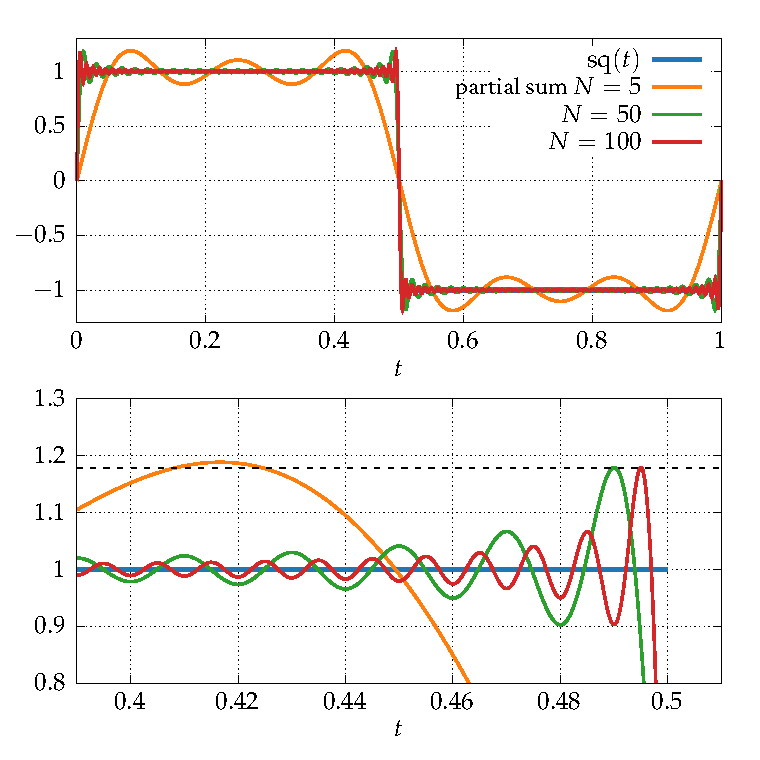
\includegraphics{gp_gibbs-sq.pdf}
  \caption{Gibbs phenomenon in the Fourier expansion of the square wave. The upper pane
    represents the square wave on one period, and its partial Fourier sum for various
    degrees. The lower pane is a zoom on the region close to the jump discontinuity at
  $t=\frac12$, and the dashed line is the excess predicted by~\cref{eq:gibbs-sq-left}.}
  \label{fig:gibbs-sq}
\end{figure}
The Fourier expansion of the square wave is illustrated in~\cref{fig:gibbs-sq}, where the
Gibbs phenomenon is clearly visible. The Gibbs phenomenon for the square wave can be
generalised to arbitrary discontinuous piecewise smooth functions, as summarised in the
theorem below.
\begin{theorem}[Gibbs phenomenon]
  Let be a $\tau$-periodic function which is piecewise smooth on $[0,\tau]$, which has a
  jump discontinuity of height $d$ at $t_0\in(0,\tau)$. Let $[a,b]$ be a sub-interval of
  $[0,\tau]$ such that $t_0\in(a,b)$, and $t_0$ is the only jump discontinuity of $f$ in
  $[a,b]$. The Fourier series of $f$ does not converge uniformly to $f$ on $[a,b]$, and
  \begin{align}
    \lim_{N\to+\infty}\,s_N(f)\left(t_0-\frac{\tau}{2N}\right)
    &=f(t_0^-)-d\left(\frac{G'}{\pi}-\frac12\right)\,,\\
    \lim_{N\to+\infty}\,s_N(f)\left(t_0+\frac{\tau}{2N}\right)
    &=f(t_0^+)+d\left(\frac{G'}{\pi}-\frac12\right)\,,
  \end{align}
  where $G'$ is the Wilbraham-Gibbs constant defined in~\cref{lem:gibbs-sq}.
\end{theorem}
%%%%%%%%%%%%%%%%%%%%%%%%%%%%%%%%%%%%%%%%%%%%%%%%%%%%%%%%%%%%%%%%%%%%%%%%%%%%%%%%%%%%%%%%%%
\section{Properties of Fourier coefficients}
%%%%%%%%%%%%%%%%%%%%%%%%%%%%%%%%%%%%%%%%%%%%%%%%%%%%%%%%%%%%%%%%%%%%%%%%%%%%%%%%%%%%%%%%%%
\section{Multidimensional Fourier series}
